\documentclass{article}

\usepackage{graphicx}

\author{Ee Xuan Tan (4907531) \and Elvira Voorneveld (4930975) \and William Narchi (5046122)}
\date{Group 40} % A small hack to add the group number AND get rid of the date
\title{Computer Graphics Project}

\begin{document}
    \maketitle

    \section{Work Distribution}
    
    \begin{tabular}{ |p{2.5cm}||p{2.5cm}|p{2.5cm}|p{2.5cm}| }
        \hline
        \textbf{Feature} &\textbf{Ee Xuan} &\textbf{Elvira} &\textbf{William}\\
        \hline
        Shading         &0\%    &100\%  &0\%\\
        Recursion       &0\%    &0\%    &100\%\\
        Hard Shadows    &0\%    &100\%  &0\%\\
        Soft Shadows    &100\%  &0\%    &0\%\\
        BVH             &40\%  &20\%    &40\%\\
        \hline
    \end{tabular}

    \section{Features}
    \subsection{Main Requirements}
    \subsubsection{Phong Shading}
    At each intersection point, the diffuse and specular terms from the Phong Model are used to calculate the lighting.
    We ignore the ambient term, as it is a crude approximation of global illumination, and therefore not necessary to incorporate.
    First, the lighting is computed separately for every light source in the scene, 
    and those results are then added together to compute the final, direct illumination.

    \begin{center}
        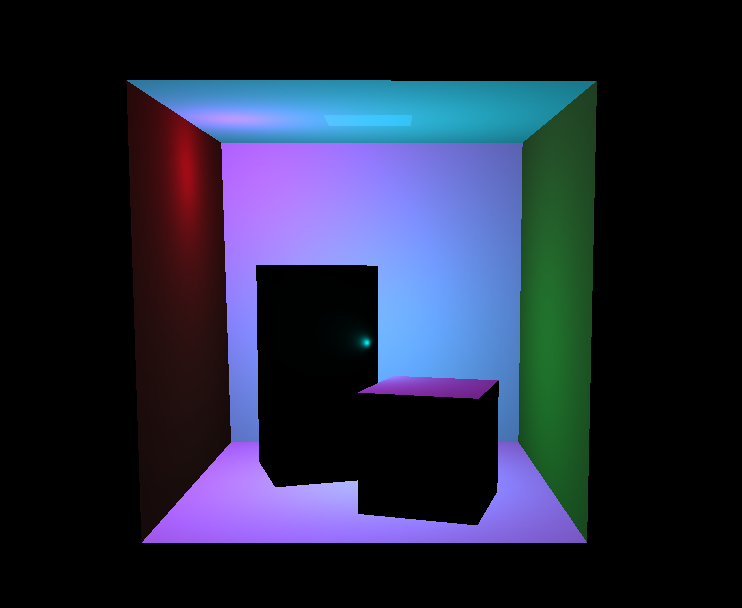
\includegraphics[scale=0.60]{images/phong_shading_showcase.png}

        The lighting effects produced by phong shading with two light sources RGB(255, 0, 255) and RGB(0, 255, 255)

        \vspace{5mm}

        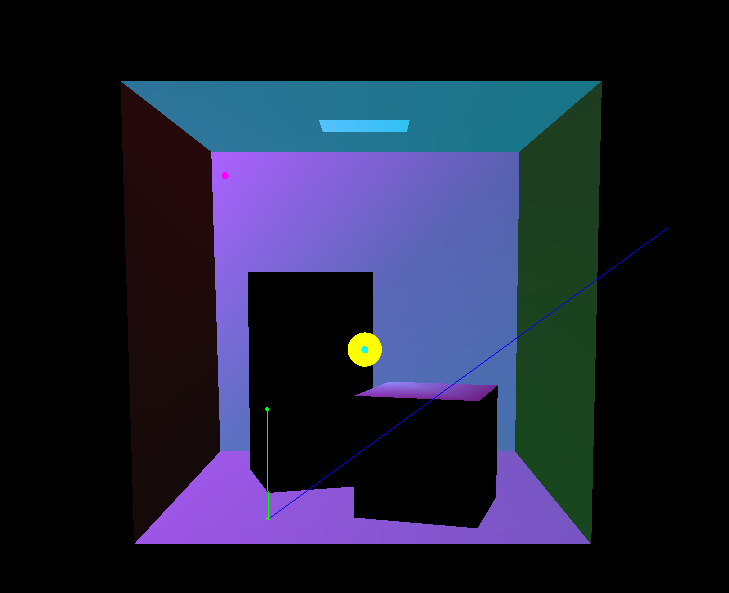
\includegraphics[scale=0.60]{images/phong_shading_debug.png}

        The phong shading debug, showing one ray shot from another angle, along with its normal
    \end{center}

    \subsubsection{Recursive Ray Tracing}
    The recursive ray tracer builds upon the previously implemented ray shading,
    creating reflection rays at each intersection point and adding the value of the reflection ray's lighting to the initial ray's specular component,
    provided that the intersection point is on a specular surface and that the reflected ray interesects a surface.
    This is done recursively until one of the previously mentioned limiting conditions applies or the recursion depth reaches a pre-set \emph{RECURSION\_LIMT}.

    \begin{center}
        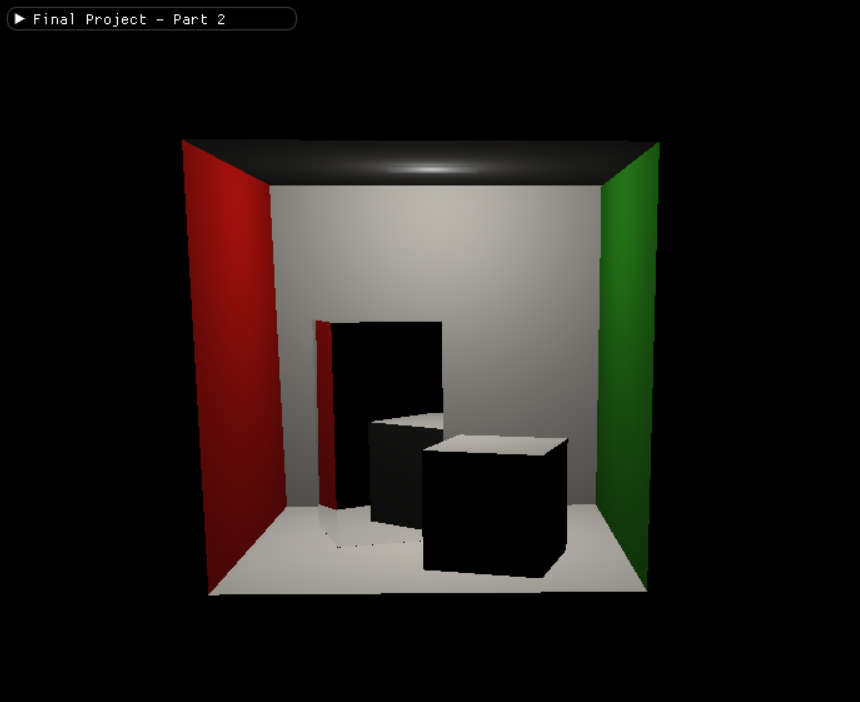
\includegraphics[scale=0.65]{images/recursive_ray_tracer_showcase.png}

        The complex specular effects produced by recursive ray tracing, which include proper mirror simulation

        \vspace{5mm}

        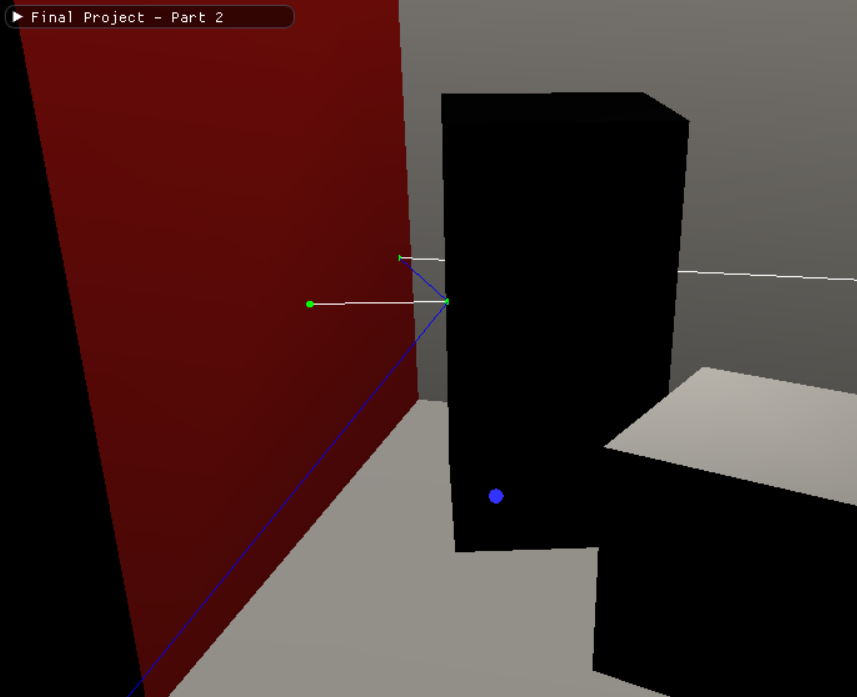
\includegraphics[scale=0.65]{images/recursive_ray_tracer_debug.png}

        The recursive ray tracer debug, showing two total rays in the recursive chain, along with their normals
    \end{center}

    \subsubsection{Hard Shadows}
    To discover which light source(s) contribute to the lighting of a certain point, ray(s) are shot from the intersection point towards the light source(s). 
    For each light source, it is computed whether or not there is a direct path between the intersection point and the respective light source. 
    Only point lights that directly shine upon the intersection point will be considered when computing the lighting in that area,
    leaving it black if none of the point lights contribute.

    \begin{center}
        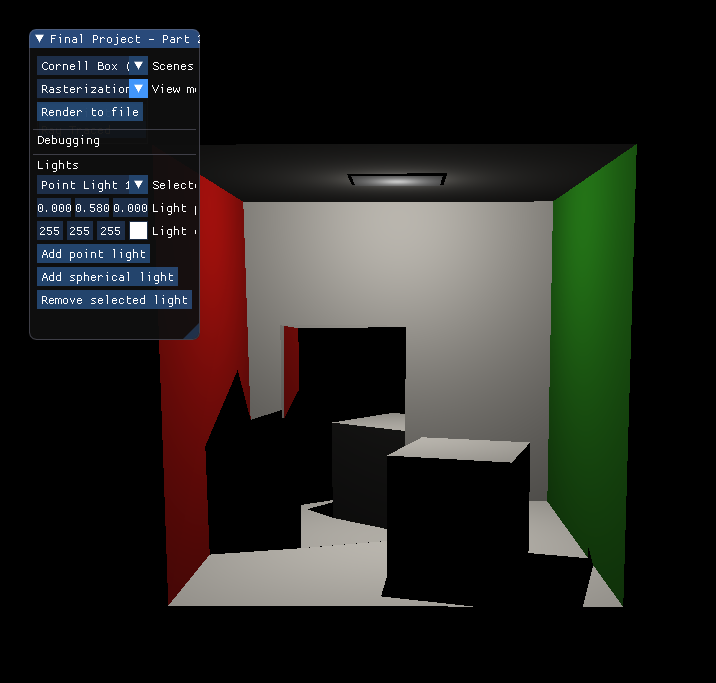
\includegraphics[scale=0.60]{images/hard_shadow_showcase.png}

        The result of using a single point light source to create hard shadows.

        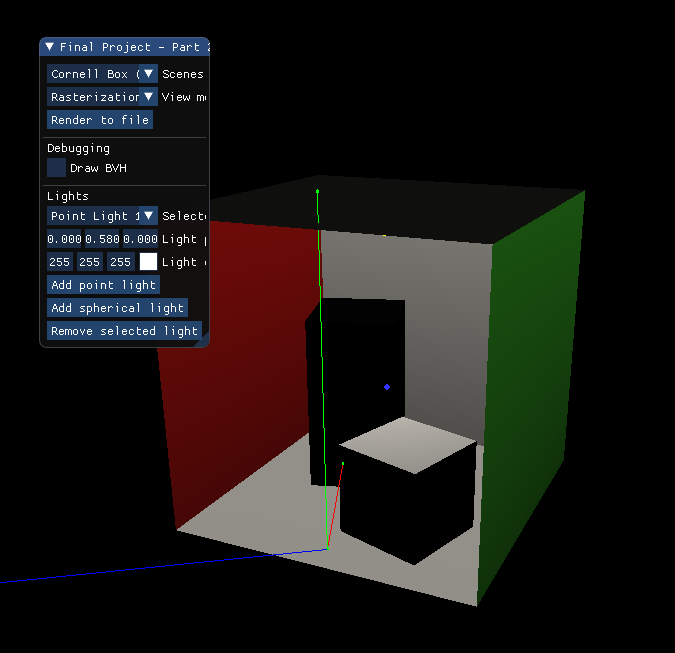
\includegraphics[scale=0.65]{images/hard_shadow_debug.png}

        The hard shadow debug, showing a ray shot from another angle, along with its normal and 
        a red line indicating the intersection with another object before reaching the point light source.
    \end{center}

    \subsubsection{Soft Shadows}
    The first step to the implementing the soft shadows is to generate uniformly distributed rays from the spherical light source. 
    In order, to get a uniform distribution of rays from the lightsource, the idea of the fibonacci sequence was used, by generating unifromly distributed 
    step sizes using the golden ratio. The second problem, was to remove light rays from the 'wrong' side of the light source, 
    this was done by using the center of the sphere and radius to calculate the longest the light ray on the 'right' side could be. 
    So, by using this method we are able to check each randomly generated sample of the light. Finally, a number of sample points are taken, 
    from these sample points we check to see if they are on the 'right' side of the sphere and if the sample ray does not intersect an object. 
    For each point we then divide the lighting value obtained by the number of sample rays taken from the sphere, giving the average light value. 

    \begin{center}
        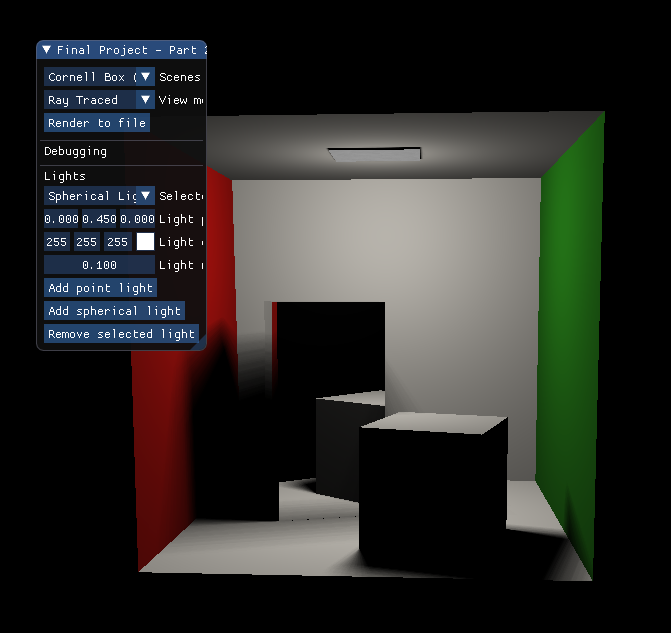
\includegraphics[scale=0.80]{images/soft_shadow_showcase.png}

        The result of using a single spherical light source with the \emph{SPHERE\_SAMPLE\_LIMIT} set to 100 to create soft shadows.

        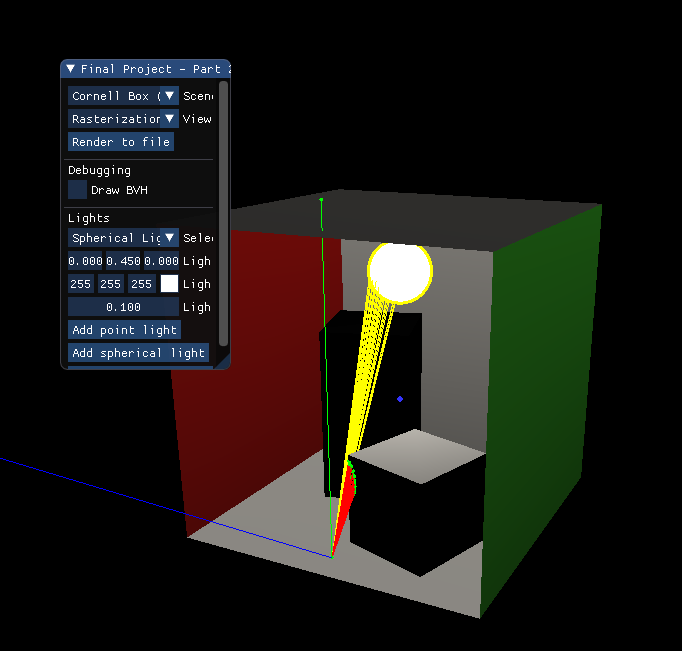
\includegraphics[scale=0.80]{images/soft_shadow_debug.png}

        The soft shadow debug, showing all of the uniformly distributed samples generated by the spherical light source.
        The yellow lines indicate a direct path from the intersection to the light source and 
        the red lines indicate the intersection with another object before reaching the spherical light source.
    \end{center}

    \subsubsection{Bounding Volume Hierarchy}
    To be constructed

    \begin{center}
        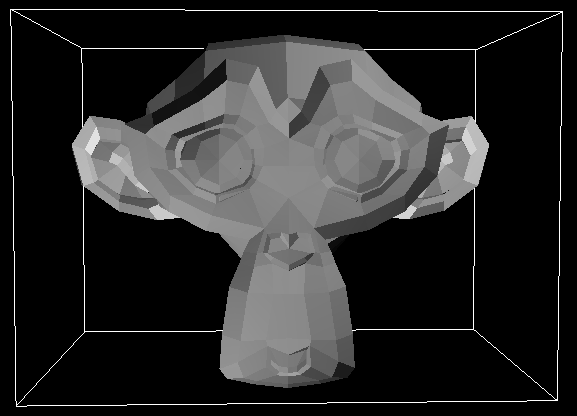
\includegraphics[scale=0.75]{images/bvh_level_one.png}

        The first level of the BVH using SAH.

        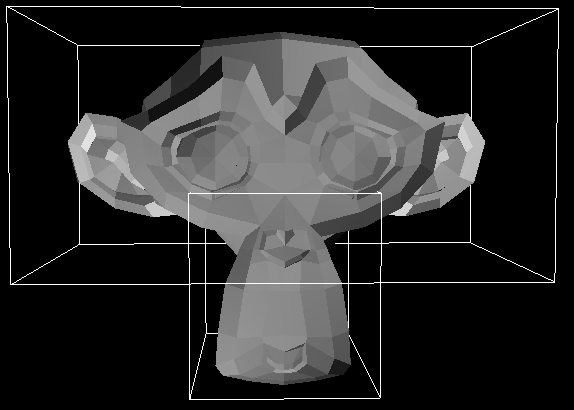
\includegraphics[scale=0.75]{images/bvh_level_two.png}

        The second level of the BVH using SAH.

        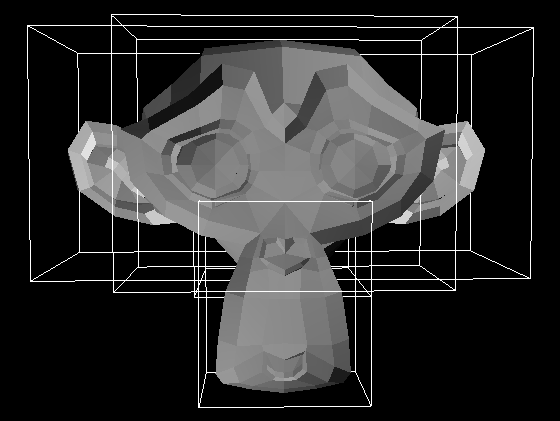
\includegraphics[scale=0.75]{images/bvh_level_three.png}

        The third level of the BVH using SAH.

        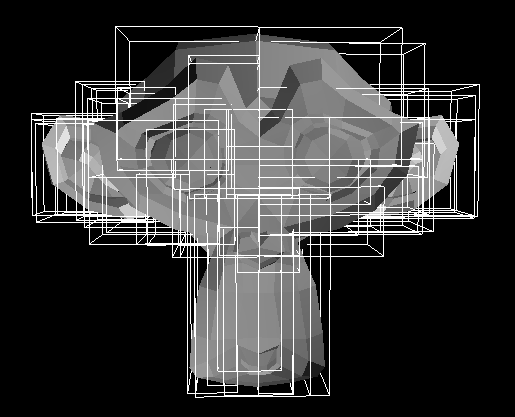
\includegraphics[scale=0.75]{images/bvh_level_ten.png}

        The tenth level of the BVH using SAH.
    \end{center}

    \section{Models}
    To be constructed

    \section{Performance Test}
    To be constructed
\end{document}
